As mentioned in \Cref{sub:subjects_objects}, three specific projects have been
selected to be used in this study. The tutorial project, designated as
YarkAdminMS\footnote{\url{https://github.com/Guergeiro/Yark-AdminMS}}, consists
of sixty-nine classes \citeSLR{brito2021identification}. Task number one
(\Cref{fig:task1_content}) utilises a Warehouse
System\footnote{\url{https://github.com/Guergeiro/Warehouse-system}} project
with a total of seventy-nine classes \citeSLR{brito2021identification}, while
task number two (\Cref{fig:task2_content}) is based on a Petclinic
System\footnote{\url{https://github.com/Guergeiro/spring-petclinic}} project
with forty classes. All of these projects are implemented in Java since,
currently, the application supports Java as the primary language for
decomposition. It is worth noting that the projects used in the study were
forked into the author's GitHub account to ensure permanent accessibility and
availability for the study.

\begin{figure*}[!htb]
  \caption{Tasks Contents}
  \centering
  \begin{subfigure}[b]{1\textwidth}
    \caption{Task 1 Content}
    \label{fig:task1_content}
    \centering
    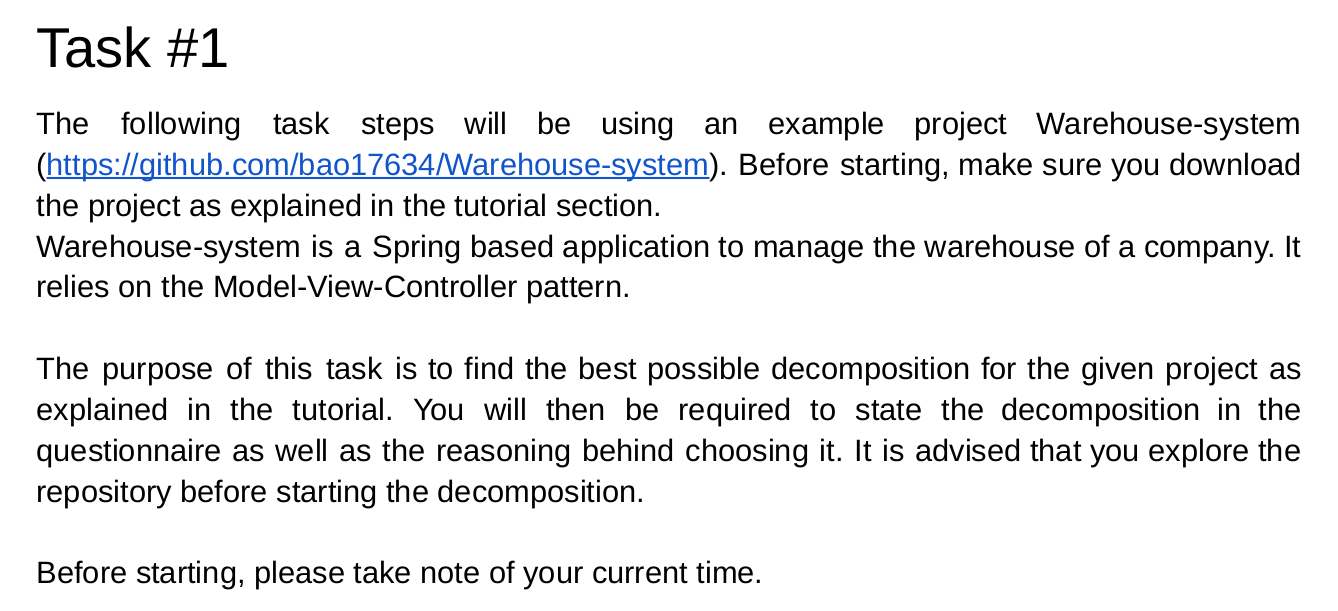
\includegraphics[width=\textwidth]{task_1}
  \end{subfigure}
  \hfill
\end{figure*}

\begin{figure*}[!htb]
  \ContinuedFloat
  \centering
  \begin{subfigure}[b]{1\textwidth}
    \caption{Task 2 Content}
    \label{fig:task2_content}
    \centering
    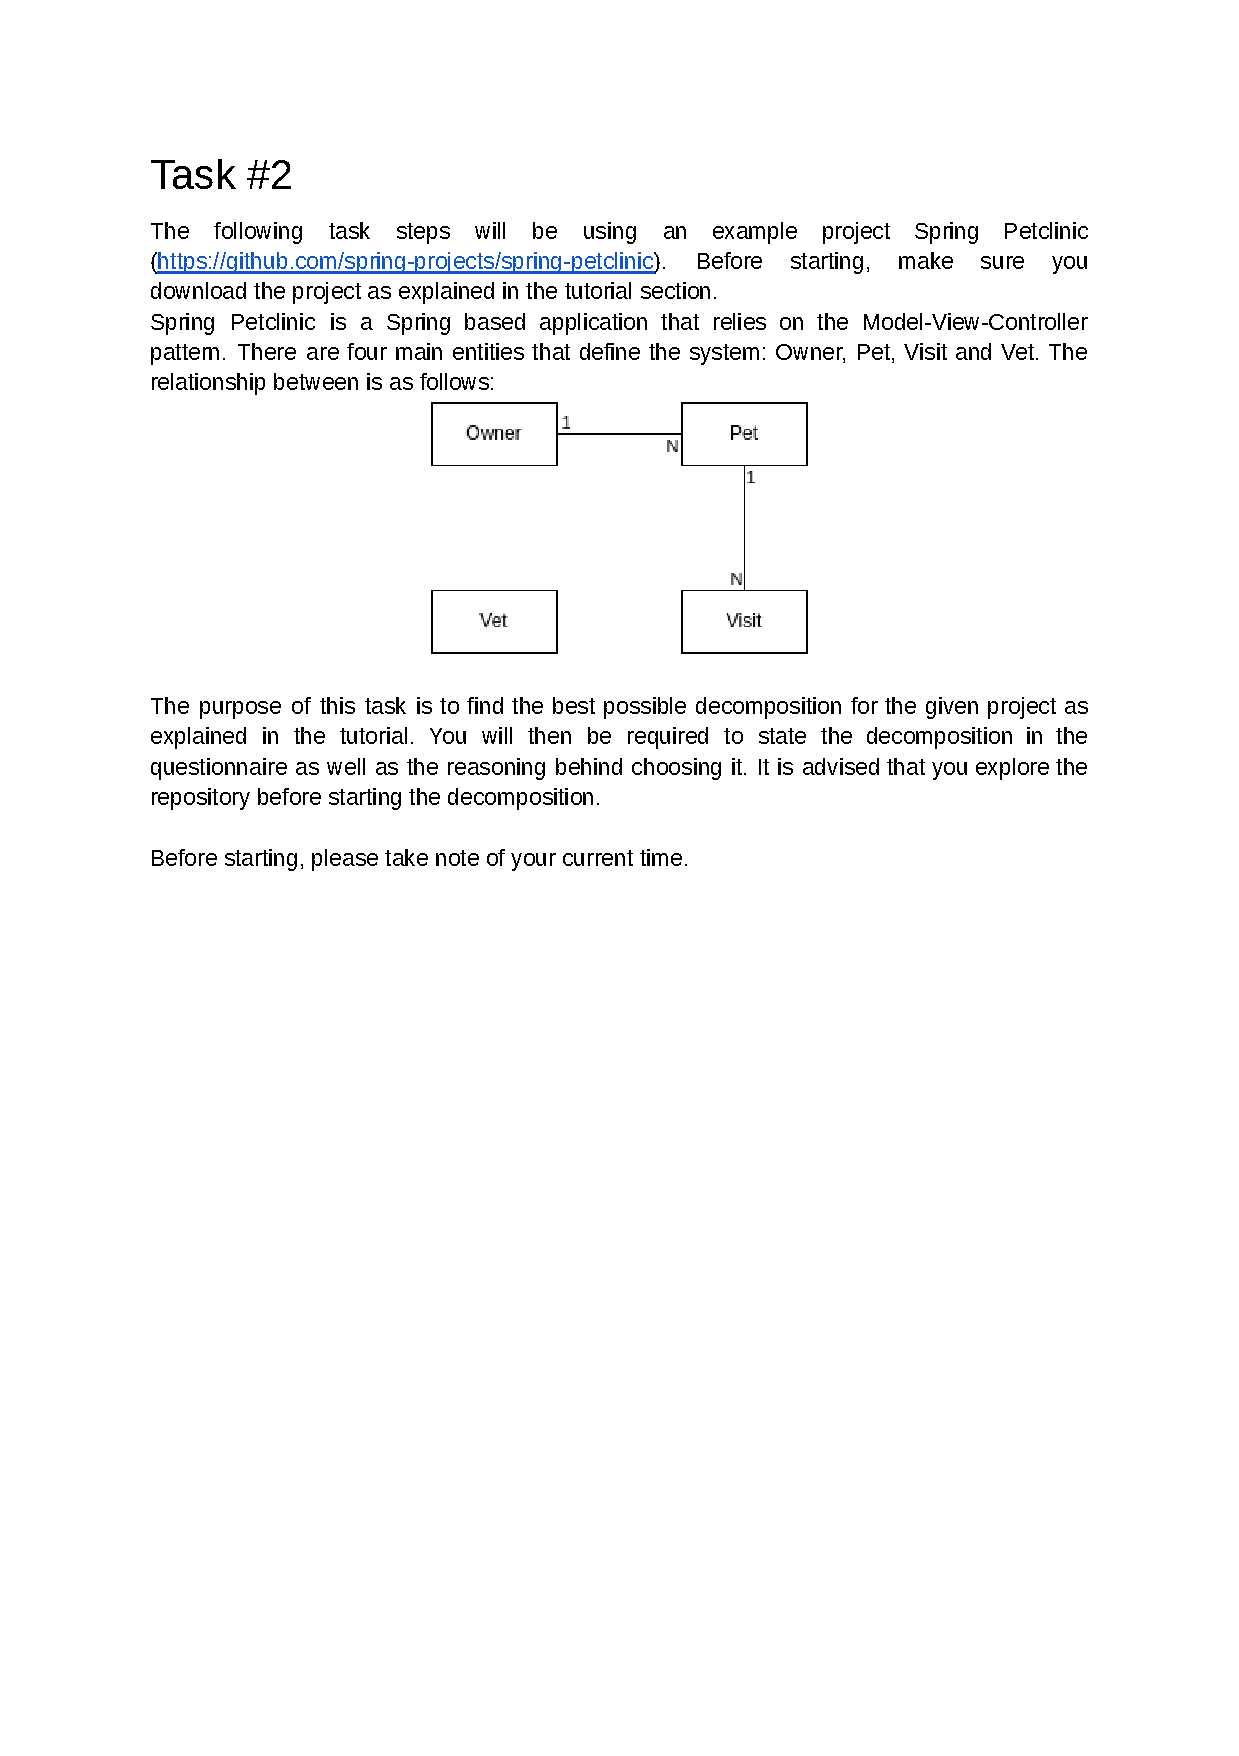
\includegraphics[width=\textwidth]{task_2}
  \end{subfigure}
\end{figure*}
